\section{Introduction}

In the last few years, we have seen the introduction of a new form of user-generated video, where severe restrictions are placed on the duration of the content. High profile examples include Vine, which allowed users to create videos up to 6.5 seconds long;  Instagram, which introduced videos up to 15 seconds duration; and Snapchat, whose videos are officially limited to 10 seconds and are deleted after 24 hours. 
Although most user-generated video platforms have placed some form of limit on the duration or size of videos (e.g., YouTube had a 10 minute limit, which has since been softened to a `default' limit of 15 mins\footnote{\scriptsize https://techcrunch.com/2010/12/09/youtube-time-limit-2/}), the extremely short duration time limits of Vine etc has led to the coining of a new term: \emph{micro videos}. 



%The most prominent example of this is the now-defunct\footnote{https://techcrunch.com/2016/10/27/twitter-is-shutting-down-vine/} platform Vine,




%On the one hand, these time restrictions offer a way for the platforms to manage the size of the videos and  thereby make the infrastructure management and content delivery more manageable \ns{Is there an evidence for this statement ? Could it be that this platform is just a market need that was never exploited?}. Thus, the time restrictions may be thought of as an artificial limit imposed on users. On the other hand, 
Some media commentators have argued that the restrictions imposed by the micro video format could fundamentally change the way we communicate~\cite{bbc}. Indeed, it has been argued that in its short lifetime, Vine has had a significant cultural impact far beyond its user base, generating several widely shared memes in its short lifetime\footnote{\scriptsize http://www.theverge.com/2016/10/28/13456208/why-vine-died-twitter-shutdown}. At the same time, as the format is still very new, virtually all major micro video platforms are experimenting with the format, making significant changes in the last year. For instance, Instagram extended the limit from 15 seconds to 1 minute\footnote{\scriptsize http://www.theverge.com/tech/2016/3/29/11325294/instagram-video-60-seconds}. Snapchat has created a new wearable, called ``Spectacles'':  sunglasses fitted with cameras that allow users to create and post 10-second long videos on the Snapchat platform\footnote{\scriptsize https://www.spectacles.com/}. 
Vine is undergoing a major overhaul -- Twitter recently said it would close down the Vine website and community. The new version of the Vine app retains the 6.5 second video format, but the videos will be published directly on Twitter's feed and thus more closely integrated with its social network\footnote{\scriptsize http://www.theverge.com/2017/1/5/14175670/vine-shutting-down-rebrand-download-archive}. 

Our goal is to understand and shed light on the salient features of this evolving medium: How do micro videos differ from other user generated videos (e.g., on YouTube)? How does the strict time limit impact video quality, and user engagement (both as creators and consumers) with such videos? %And as a corollary, do longer time limits change quality or user engagement?
 What are the relative roles of  social and content quality factors in driving engagement and popularity -- Is Vine's anticipated integration with the Twitter social network and feed well motivated? 

We answer these questions from an empirical perspective, using a dataset of nearly all ($\approx 120,000$) Vine videos that were uploaded to one of the 18 globally available channels on Vine during an 8 week period. We complement these with other datasets including a curated dataset (\emph{POP12K}) of 12,000 popular Vine videos, as well as samples from other platforms -- Instagram, Flickr and YouTube\footnote{Flickr and YouTube data are publicly shared. On acceptance, our newly crawled data will also be shared  for non commercial research}.
 
%The paper then takes a first look at how users engage with micro videos, 
 %and also a platform with one of the shortest time duration restrictions (just over 6 seconds).
 
%We take an empirical approach, and crawl the Vine platform to collect POP12K, a dataset of about 12,000 videos which have been deemed by Vine to be popular, and therefore, by definition, have engaged a large number of users. We complement this by collecting ALL120K, a dataset of nearly all ($\approx$ 120,000)  videos that were uploaded to one of the 18 globally available channels on Vine during an 8 week  period. %For a broader scope, we reverse engineer the Instagram user search API and do a search based crawl of instagram users. 
%  For each video in our datasets\footnote{Both datasets will be shared for non-commercial research.}, we derive 28 aesthetic and affect (sentiment)-related features (Refer to Table \ref{tab:Features_table}) both from the visual and audio tracks, and collect statistics of the number of times each Vine was looped through, reposted or `revined', and liked by different users. 


%%%%

% Similarly, David Pogue, writing in the Scientific American, conjectured that micro videos are a whole new form of expression more closely related to images than to videos~\cite{pogue13}:
%\begin{quotation}
%	A photograph is intended to capture a single moment, to present it for thoughtful examination. In the end, that's what a one- or six-second looping video does so well -- it's just that it expands the scope of the still image \ldots Maybe the micro video is best considered an improvement on a still picture, not a downgrade from video.
%\end{quotation}
%
%This  hypothesis raises the question of whether it is only \emph{conceptually} convenient and interesting to model  micro videos as enhanced images, or whether users also \emph{engage} \footnote{Throughout this work, we use Engagement and Popularity interchangeably as we treat them as such interdependent.} with micro videos in ways similar to images. The answer has strong implications for how micro video platforms are designed and used. For instance, advertisements in videos carry a higher price than other media. From the perspective of users, an image-like medium may benefit from image-like editing tools such as filters, cropping, fitting etc, whereas a video-like medium would benefit from non-linear or multi-track editing features. %More importantly, many micro video platforms have started relaxing the time restrictions (e.g., Instagram videos can now last up to 60 seconds, and Vine recently introduced an option where users can attach a longer video up to 140 seconds long that can be reached in a single click from the 6 minute micro video). 
%If in fact users see value in micro videos as images with embedded live action, then such attempts may alter  the very 	e of the medium of expression. 

%%%%

%This paper first tries to hint at the phenomenon of shorter videos being a preferred and more so an effective engagement medium by studying two popular social media networks, namely Vine and Instagram. 

Using these datasets, we systematically examine the nature of user engagement in Vine on three levels. First, we compare the features of micro videos in \emph{POP12K} with corresponding features of popular content on image-based and video-based user generated content platforms (Flickr and YouTube respectively) and find for the first time quantitative evidence that lends support to David Pogue's theory of micro videos as a whole new form of expression falling on a spectrum between images and videos~\cite{pogue13}. 

Next, we take the three metrics of popularity we collect -- counts of loops, reposts and likes -- as quantification of the \emph{collective} user engagement of the consumers of a video, and ask to what extent the content- and social network-related features affect these metrics. To answer this question, we adopt a novel methodology.
We train a random forest classifier that, given a threshold for a metric of popularity, is able to able to distinguish items on either side of the threshold into popular and unpopular classes  with high accuracy, precision and recall, using the features we have identified. The relative importance of different features then gives an indication of the extent to which those features affect the metric under consideration. We progressively consider higher and higher threshold values for videos to qualify as popular or engaging, and thereby identify trends and changes of relative importance of different features. Interestingly, we find that as the threshold for popularity becomes more and more stringent, features that represent quality of the content become collectively as important as social features such as the number of followers. Echoing an effect also observed in Instagram photos~\cite{bakhshi2014faces}, we find that presence of faces significantly increases engagement, and is the most important content-related factor.

Finally, we ask how these features vary over time in micro-videos, and discover a \emph{primacy of the first second} phenomenon: the best or most salient parts of the video, whether in the aesthetic space or affect space, are more prevalent in the initial seconds of the micro video, suggesting that the authors are consciously or unconsciously treating micro-videos similar to images -- in the initial part, the video is composed with aesthetics and affective quality in mind, resulting in a higher quality level; but quality declines as the video plays over time. Furthermore, echoing the primacy of the first second phenomenon, we find that the quality of the first seconds of the video are as effective as the quality of the whole video in predicting popularity/engagement. Fig.~\ref{fig:Vine_samples} shows examples of these effects through two videos in our dataset of popular videos. In both videos, we observe content quality deteriorate over time, illustrating the primacy of the first seconds. 
 
\begin{figure}[!tbh]
\centering
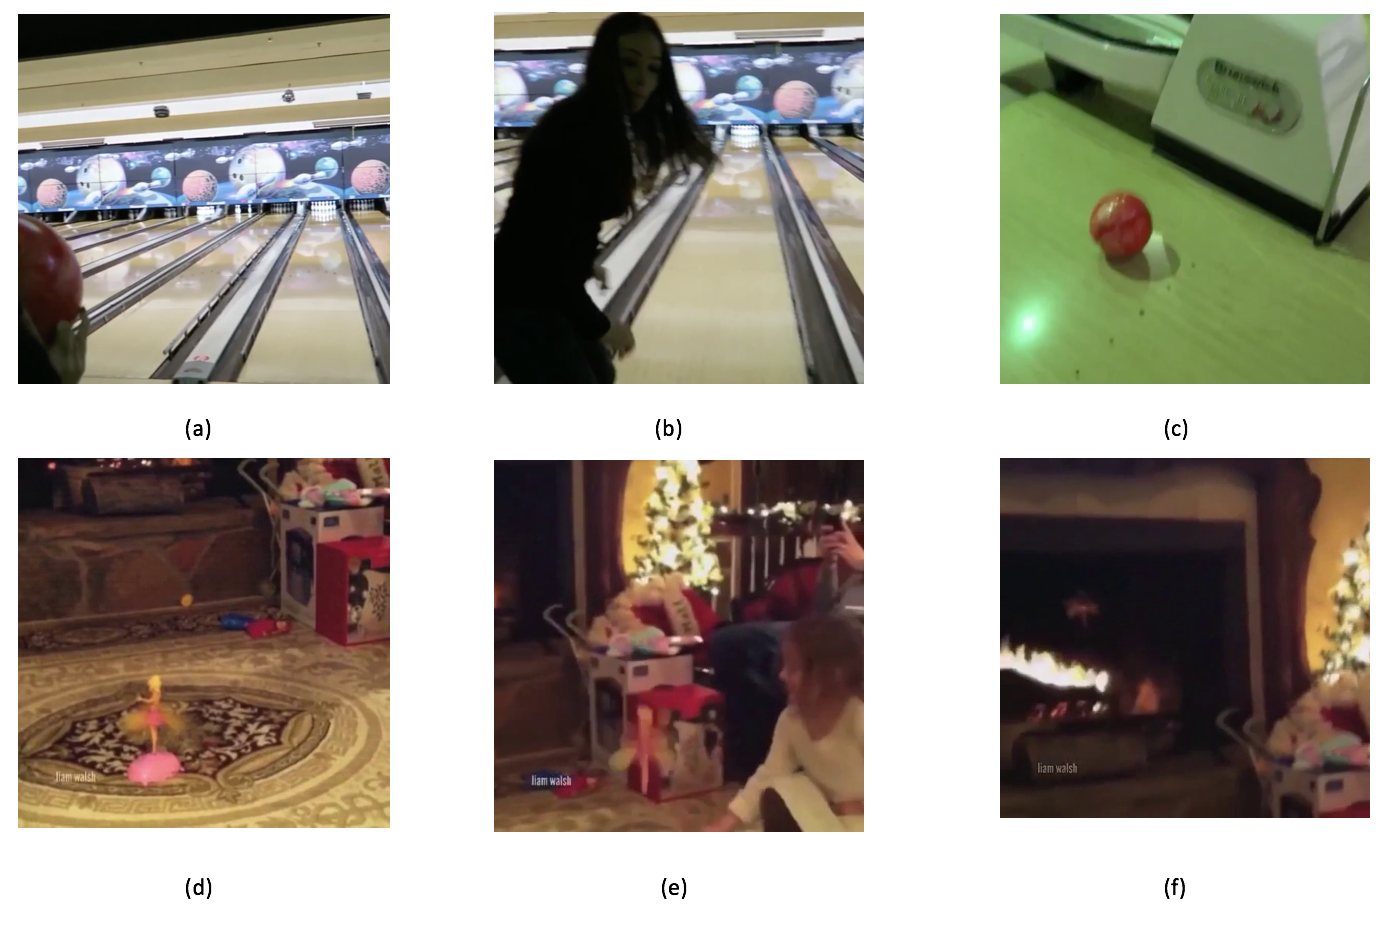
\includegraphics[width=\columnwidth]{figures/Vine_samples2}
\caption{\textsl{ Vine Samples from first, second and thirds one thirds of the video. Images (a) , (b) and (c) show a progressive drop in brightness and sharpness due to shaky camera. Images (d) (e) and (f) shows a progressive drop in contrast.}}
\label{fig:Vine_samples}
\end{figure}
%
%
%novel concept of a popularity classifier that is able to accurately distinguish popular and unpopular items for varying definitions of popularity. 
%We develop a simple random forest classifier that is able to distinguish popular and unpopular items with high accuracy, for varying definitions of popularity. 
%
%
  %The  only exception is the prevalence of faces -- the presence of faces is the single most important content-related feature that makes a vine popular, and popular videos have a  higher fraction of frames with faces in them; thus later frames also matter if the frames contain faces. 


%The rest of the paper is structured as follows: \S\ref{sec:dataset}...



%\hrule
%
%\textbf{Below this is construction material for elsewhere}
%As with other user-generated content, users may engage either as \emph{producers} of content or as \emph{consumers}. 
%
%User engagement is both what users see and what they feel (cite). So we look at aesthetics as well as affect. Information comes in three channels: audio, video and sentiments. Vine engagement can be understood in terms of consumers and producers: what users produce and how they produce it. 
%
%We examine this question in three 
%
%the time restrictions shape user engagement with micro videos. To this end, we chose to examine Vine, one of the earliest and most popular micro video platforms, and also a platform with one of the shortest time duration restrictions (just over 6 seconds). We start by crawling POP12K, a dataset of about 12,000 videos which have been deemed by Vine to be popular, and therefore, have by definition, engaged a large number of users. We complement this by collecting ALL120K, a dataset of nearly all ($\approx$ 120,000)  videos that were uploaded to one of the 18 globally available channels on vine.
%
%To understand which aspects impact engagement, we look at both the video and audio signals in the micro video. We consider \emph{aesthetics} -- how well constructed the video is, as well as affect -- the emotions the video can evoke. We ask if we can distinguish ``popular'' videos from the unpopular ones based on these different signals, and find that surprisingly, we can do a great
%
%We first compare the popular micro videos in POP12K with popular user-generated images from Flickr and user-generated videos from YouTube, and find that micro videos appear to occupy a middle ground between images and videos. Then we ask whether and to what extent the

%In an age when 
%
%The Art of story telling could be attributed to be one of the most ancient arts. It could be in the form of neolithic paintings to the egyptian hieroglyphs or among the elaborate epics of Illiad and oddyssey to the elaborate power plays of the Game of thrones, humans have always strived to record or create elaborate plots and stories. The human need of transferring experiences to others in different forms of creative arts, has ever so created the world as interesting as we see it. 
%\par
%The art of story telling has spawned and transformed several industries, including the very important entertainment industry. With progress of technology, entertainment industry has gone through several rejuvination cycles. Starting with plays to television, each technological advancement has created a new form of stories to be presented. The latest of these cycles was powered by the internet with the help of services like Youtube, Netflix, Hulu and Amazon. 
%
%\par
%Over the past few years, the idea of microvideos has taken over the social world. It started with Vine, a company that was found in 2012, which allowed users to upload micro videos, not larger than 6 seconds. These videos are then consumed and shared, and are ranked based on how many times they are looped over. The videos have a spectrum of generes, starting from a quick home video about domestic cats and dogs, to elaborate short skits done by now acclaimed vine stars 
%
%\footnote{www.vanityfair.com/hollywood/2016/02/king-bach-rocketjump-youtube-vine-stars}
%\footnote{http://newmediarockstars.com/2015/04/youtubers-viners-attend-the-white-house-correspondents-dinner-gallery/}conceive of micro vuch as w